\documentclass{beamer}

\usepackage[utf8]{inputenc}
\usepackage[russian]{babel}

\usepackage{graphicx}
\usepackage{gensymb}

\usefonttheme[onlymath]{serif}

%\usepackage{beamerthemesplit}
%\useoutertheme{infolines}
%\useoutertheme{smoothtree}
\useoutertheme{tree}
\useinnertheme{circles}
\setbeamertemplate{itemize items}[default]
\setbeamertemplate{enumerate items}[default]

\definecolor{myblue}{rgb}{.0,.2,.3}
\setbeamercolor*{palette primary}{use=structure,fg=white,bg=myblue}
\setbeamertemplate{navigation symbols}{}

\usepackage{tikz}
\usetikzlibrary{shapes.geometric, arrows, trees}
\tikzstyle{every node}=[font=\tiny, node distance=0.8cm]
\tikzstyle{io} = [trapezium, trapezium left angle=70, trapezium right angle=110, minimum width=1cm, minimum height=0.33cm, text centered, text width=1cm, draw=black, fill=blue!30]
\tikzstyle{process} = [rectangle, minimum width=1cm, minimum height=0.31cm, text centered, draw=black, fill=orange!30]
\tikzstyle{decision} = [diamond, minimum width=1cm, minimum height=0.31cm, text centered, draw=black, fill=green!30]
\tikzstyle{arrow} = [thick,->,>=stealth]
\tikzstyle{bigrect} = [rectangle, minimum width=5.5cm, minimum height=4.5cm, text depth=5cm, draw=black, dashed]

%\usepackage{verbatim}
\usepackage{listings}
%\usepackage{enumitem}
%\setlistdepth{9}
%\setlist[itemize,1]{label=$\bullet$}
%\setlist[itemize,2]{label=$\bullet$}
%\setlist[itemize,3]{label=$\bullet$}
%\setlist[itemize,4]{label=$\bullet$}
%\setlist[itemize,5]{label=$\bullet$}
%\setlist[itemize,6]{label=$\bullet$}
%\setlist[itemize,7]{label=$\bullet$}
%\setlist[itemize,8]{label=$\bullet$}
%\setlist[itemize,9]{label=$\bullet$}
%\renewlist{itemize}{itemize}{9}

\newcommand{\layersInRealLife} {
  \frametitle{Уровни (levels / layers) в реальной жизни}
  \framesubtitle{Уровни характеризуются \textbf{обязанностями} и определяют \textbf{кто над кем главнее (выше)}}

  \begin{itemize}
    \item Директор конторы (высокий уровень)
      \begin{itemize}
        \item Художник (низкий уровень)
        \item Программист (низкий уровень)
        \begin{itemize}
          \item Младший программист (самый низкий уровень)
        \end{itemize}
      \end{itemize}
  \end{itemize}
}

\newcommand{\paradigmsImpDecl} {
  \node (imper) [bigrect, xshift=-1cm] {Императивное};
  \node (decl) [bigrect, xshift=5cm, yshift=2.5cm] {Декларативное};
}

\newcommand{\paradigmsAlg} {
  \paradigmsImpDecl

  \node (alg) [process, dashed, xshift=-1cm, yshift=1cm] {Алгоритмическое};
    \node [xshift=-1cm, yshift=0.65cm] {Блок-схемы, словесное описание};
}

\newcommand{\paradigmsStruct} {
  \paradigmsAlg

  \node (struct) [process, xshift=0cm, yshift=0cm] {Структурное};
    \node [xshift=0cm, yshift=-0.35cm] {Ограничение алгоритмического};
  \draw [arrow] (alg) -- (struct);
}

\newcommand{\paradigmsProc} {
  \paradigmsStruct

  \node (proc) [process, xshift=-1cm, yshift=-1cm] {Процедурное};
    \node [xshift=-1cm, yshift=-1.35cm] {C, Pascal...};
  \draw [arrow] (struct) -- (proc);
}

\newcommand{\paradigmsOop} {
  \paradigmsProc

  \node (oop) [process, xshift=-1.5cm, yshift=-2cm] {Объектно-ориентированное (ООП)};
    \node [xshift=-1.5cm, yshift=-2.35cm] {C++, C\#, Java, Python, Ruby, JS, ...};
  \draw [arrow] (proc) -- (oop);
}

\newcommand{\paradigmsDecls} {
  \paradigmsOop

  \node (notprog) [process, dashed, xshift=5cm, yshift=4cm] {Описания};
    \node [xshift=5cm, yshift=3.65cm] {Конфигурации и Web API (XML, JSON),};
    \node [xshift=5cm, yshift=3.35cm] {вёрстка (HTML, LaTeX), аннотации};
}

\newcommand{\paradigmsFunc} {
  \paradigmsDecls

  \node (func) [process, xshift=4cm, yshift=2.5cm] {Функциональное};
}

\newcommand{\paradigmsLogical} {
  \paradigmsFunc

  \node (logical) [process, xshift=5cm, yshift=1cm] {Логическое};
}

\newcommand{\paradigmsAll} {
  \paradigmsLogical

  \node (generic) [process, xshift=-1cm, yshift=5cm] {Обобщенное};
  \node (concurrent) [process, xshift=5cm, yshift=-2cm] {Конкурентное};
  \node (module) [process, xshift=-2cm, yshift=4cm] {Модульное};
}


\title{Введение в программирование}
\author{Лопатин Александр}
\date{2015}


\subtitle{Лекция 2}

\begin{document}

  \frame{\titlepage}


  \section*{Содержание} {
    \frame{\tableofcontents[hideallsubsections]}


  \section{Языки программирования}
    \frame {
      \frametitle{Язык программирования}
      Знаковая система \underline{для написания компьютерных программ}

      \vspace{0.5cm}
      Текст, написанный на таком языке называют \underline{текст программы} или \underline{исходный~код}~(source~code) или просто \underline{код}
    }

    \frame {
      \frametitle{Трансляторы языков программирования}
      Программы, которые \underline{понимают исходный код}

      \vspace{0.5cm}
      Бывают двух типов:
      \begin{itemize}
        \item Компилятор --- превращает текст программы в \underline{двоичный код}
        \item Интерпретатор --- читает текст программы и выполняет написанное
      \end{itemize}
    }

    \frame {
      \frametitle{Двоичный код}
      \begin{itemize}
        \item \textbf{машинный код} (machine/native code) --- код, который исполняет \underline{аппаратный} исполнитель (например микропроцессор)
        \item \textbf{байт-код} \underline{виртуальной машины} --- код, который исполняет \underline{программный} исполнитель (например <<виртуальная машина .NET>> или <<виртуальная машина Java (JVM)>>) 
      \end{itemize}

      \vspace{0.5cm}
      Понятие <<виртуальная машина>> --- многозначно.
      Об этом разжевано здесь:
      \url{http://habrahabr.ru/company/intel/blog/254793/}
    }

    \frame {
      С ростом популярности \underline{JIT-компиляции} разделение \underline{трансляторов} на
      \underline{компиляторы и интерпретаторы} не столь актуально

      \vspace{1cm}
      Большинство \underline{актуальных интерпретаторов} стало, грубо говоря,
      \underline{компиляторами} в \underline{машинный код})

      \vspace{1cm}
      \url{https://ru.wikipedia.org/wiki/JIT}
    }

    \frame {
      Лучше разделять сами языки, а не трансляторы:
      \begin{itemize}
        \item \textbf{Компилируемые} (Assembler, C++, C\#, Java, ...)
        \item \textbf{Скриптовые} (Python, Ruby, JavaScript/ECMAScript, bash/shell, cmd/bat, PowerShell, ...)
      \end{itemize}
    }

    \frame {
      \frametitle{Компилируемые языки}
      Исходный код компилируют в \underline{двоичный код} и (обычно) распространяют в скомпилированном виде (.exe, .jar, .dll и т.д.)

      \vspace{0.5cm}
      Часто используется для:
      \begin{itemize}
        \item \textbf{прикладного программирования} (от текстового редактора до веб-браузера или более сложной системы)
        \item \textbf{системного программирования} (драйвера устройств и т.д.)
      \end{itemize}
    }

    \frame {
      \frametitle{Скриптовые языки (языки сценариев)}
      \framesubtitle{Для многих --- синоним к <<Интерпретируемым языкам>>}
      Программы обычно распространяют в виде исходного кода (.py,~.js,~.bat~и~т.д.)

      \vspace{0.5cm}
      Часто используется для:
      \begin{itemize}
        \item \textbf{прототипов} прикладных программ
        \item \textbf{сценариев} для автоматизации: сборка/тестирование билда, deploy на сервер
        \item \textbf{плагинов/расширений} (для браузера, скажем)
        \item клиентский или серверный \textbf{код для веб-сайта}
      \end{itemize}

      \vspace{0.5cm}
      Популярно там, где хочется \underline{быстро увидеть результат}
    }

    \frame {
      А еще языки классифицируют по тому, на какие \textbf{парадигмы~программирования} сделан основной акцент...
    }

    \frame {
      \frametitle{Wait, wait...}
      \framesubtitle{Зачем об этом всём знать? Для осознания того}

      \begin{itemize}
        \item что языки можно \underline{очень по-разному} классифицировать
        \item \underline{одни классы} эффективно решают \underline{одни типы задач}, другие классы --- другие типы задач
        \item{} <<универсального>> языка \underline{не существует}
        \item чем более \underline{узкоспециализирован} язык (SQL для БД, G-Codes для станков, ...) или комбинация языка и фреймворка (Ruby+RoR или JS+node.js для веб) тем \underline{быстрее} их можно изучить
      \end{itemize}

      Другими словами --- чтобы знать по какому принципу выбирать следующий язык для изучения

      \vspace{0.5cm}
      \url{https://www.youtube.com/watch?v=LR8fQiskYII}
      \url{https://www.youtube.com/watch?v=NvWTnIoQZj4}
    }

    \frame {
      \frametitle{На википедии}
      Можно увидеть разницу между языками, если обращать внимание на \underline{Paradigm} и \underline{Typing discipline}
      \begin{center}
        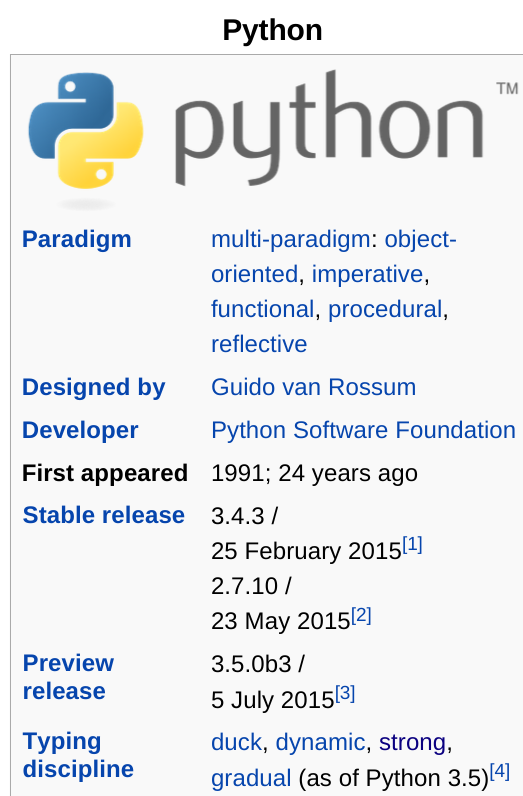
\includegraphics[scale=0.18]{pictures/python.png}
        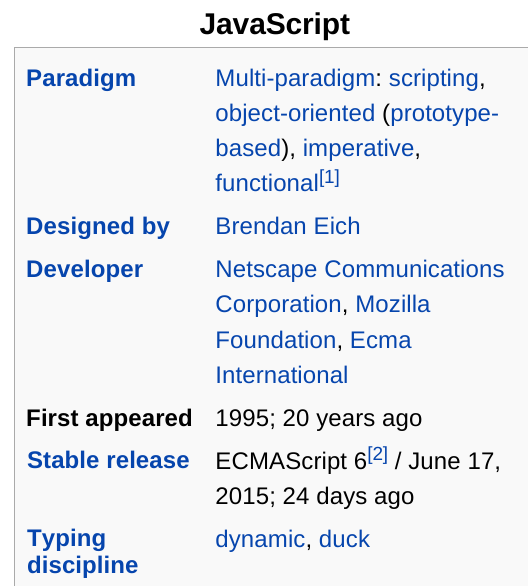
\includegraphics[scale=0.2]{pictures/js.png}
        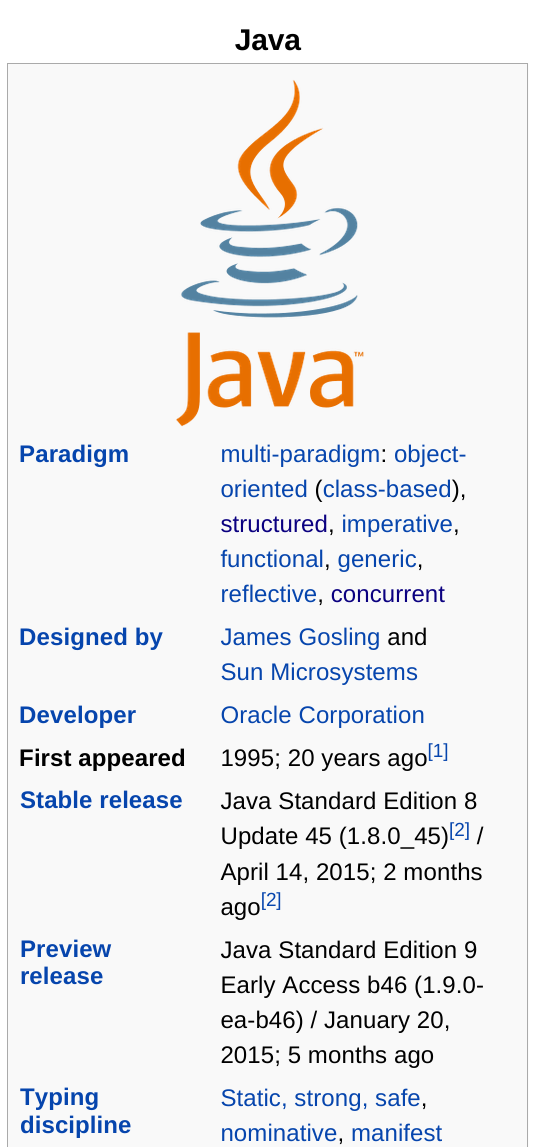
\includegraphics[scale=0.12]{pictures/java.png}
      \end{center}
    }
\end{document}
